% -*-cap1.tex-*-
% Este fichero es parte de la plantilla LaTeX para
% la realización de Proyectos Final de Carrera, protejido
% bajo los términos de la licencia GFDL.
% Para más información, la licencia completa viene incluida en el
% fichero fdl-1.3.tex

% Copyright (C) 2009 Pablo Recio Quijano 



\section{Introducción}
\nombrejuego es un videojuego en 2D del género de las aventuras gráficas, con una ambientación en la Cádiz actual cuyo objetivo es tanto de entretener al jugador como que aprenda anécdotas y hechos relacionados con Cádiz en los años que fue asediada y vieron nacer la Constitución de 1812. Dicho videojuego hace uso de \programa{Unity3D}, un motor de desarrollo de videojuegos multiplataforma. 

En \nombrejuego controlaremos a un estudiante de la Licenciatura de Historia de la Universidad de Cádiz, que recientemente ha suspendido un examen y va al despacho a pedir una revisión para su nota. Sin embargo, no logra encontrar al profesor y se embarcará en una aventura para descubrir el paradero de dicho profesor ayudándose de las pistas obtenidas al resolver puzzles teniendo estos siempre una relación con la Cádiz de 1812. El videojuego tiene que estar completamente documentado, pues una gran gran parte de la jugabilidad y de la parte educativa del juego, recae completamente en el buen diseño que se haga de los puzzles, estancias e interacciones con otros personajes no controlables.

Con todo esto se pretende demostrar que un videojuego se puede usar de material didáctico en entidades educativas de todos los ámbitos, y promover el contenido interactivo sin olvidarse del entretenimiento como manera de aprendizaje para jugadores de cualquier edad.

\section{Contexto}
\label{sec:contexto}

[...]

\subsection{Historia del auge, caída, y resurgir de las aventuras gráficas}
\label{sec:ag}
La aventura gráfica es un subgénero de los videojuegos de aventura. Su mecánica consiste en ir avanzando por el mundo, escenario o juego a través de la resolución de diversos puzzles, planteados como situaciones que se suceden en la historia, interactuando con personajes y objetos a través de un menú de acciones o interfaz similar, utilizando un cursor para manejar al personaje y realizar las distintas acciones. En su concepción clásica, esta siempre incluía la visión de los personajes en tercera persona, aunque en varias ocasiones se planteasen en primera persona. 

Este género se originó a partir de las aventuras conversacionales anteriores a los años 80. Era una época en la que los ordenadores personales aún carecían de gráficos y sólo se podía interactuar con ellos escribiendo líneas de comandos a lo que te contestaban en texto. 

Como se estaban instaurando con éxito en los hogares, pronto hubo gente que se dedicó a buscar un nuevo abanico de entretenimiento y ocio basado en ellos. De ellos nacieron las aventuras conversacionales, la primera de ellas fue Colossal Cave Adventure \cita{cave-adventure} (véase la figura ~\ref{fig:text-adventure}). En estos la acción se desarrollaba describiendo en un párrafo la situación actual del protagonista y abajo un cuadro de texto en el que había que escribir sencillas frases para interactuar con el entorno, del tipo ``hablar con el anciano'', ``usar llave'', ``salir por la puerta'' o indicando puntos cardinales para ir de un sitio a otro, como por ejemplo ``norte'' o ``sur''.

\begin{figure}[H] 
  \begin{center}
    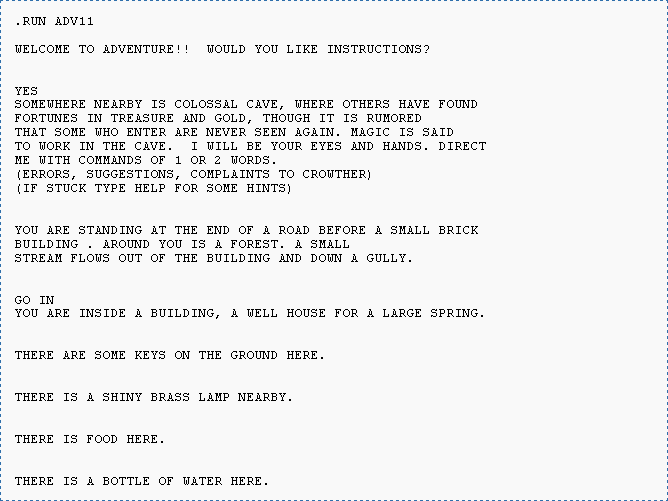
\includegraphics[scale=0.5]{first-text-adventure.png}
  \end{center}
  \caption{Colossal Cave Adventure (PDP-10, 1977), la primera aventura conversacional}
    \label{fig:text-adventure}
\end{figure}

No fue hasta en 1980, en la que la compañía Online System (que más tarde pasó a llamarse Sierra Online \cita{sierra-online}) creó la primera aventura gráfica propiamente dicha. Este juego con gráficos rudimentarios era Mystery House \cita{mystery-house} (Apple II, 1980) (veáse la figura ~\ref{fig:mystery-house}), luego le siguió Wizard and the Princess \cita{wizard-princess} (Apple II, 1980) ya con gráficos en color, y finalmente establecieron el género con King's Quest \cita{king-quest} (Apple II, 1984) con su aparición en varios sistemas y asentándose en la industria con cada vez títulos más fuertes.

\begin{figure}[H] 
  \begin{center}
    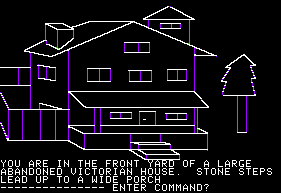
\includegraphics[scale=1]{mystery-house-first-graphic-adventure.png}
  \end{center}
  \caption{Mystery House, la primera aventura con gráficos}
  \label{fig:mystery-house}
\end{figure}

El lanzamiento del Apple Macintosh y su interfaz controlada por ratón supuso la creación de las aventuras gráficas \cursiva{point-and-click}, introduciendo a más empresas a este mercado. LucasArts \cita{lucasarts} fue una de ellas, la cual consiguió un éxito rotundo con su primer juego, Maniac Mansion (veáse la figura ~\ref{fig:maniac-mansion}) \cita{maniac-mansion}, con una interfaz íntegramente \cursiva{point-and-click}, imponiéndose como otra gran empresa dentro de la industria. Mientras tanto, Sierra Online también se sumaría a este cambio pasando su sistema de introducir comandos por una rudimentaria interfaz \cursiva{point-and-click} con Manhunter: New York \cita{manhunter} (veáse la figura ~\ref{fig:manhunter}).

\begin{figure}[H] 
  \begin{center}
    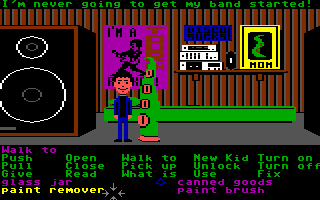
\includegraphics[scale=1]{maniac-mansion-commodore64.png}
  \end{center}
  \caption{Maniac Mansion (1987), con su interfaz exclusivamente \cursiva{point-and-click}}
    \label{fig:maniac-mansion}
\end{figure}

\begin{figure}[H] 
  \begin{center}
    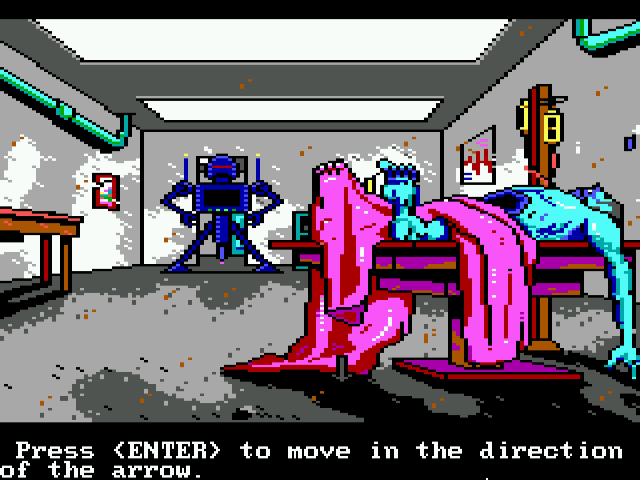
\includegraphics[scale=0.7]{manhunter.png}
  \end{center}
  \caption{Manhunter: New York (1989), con una interfaz \cursiva{point-and-click} primitiva con teclas}
    \label{fig:manhunter}
\end{figure}

Sierra Online y LucasArts seguían un camino lleno de rivalidades la una con la otra, aunque cada una seguiría su propio camino:
\begin{itemize} 
\item Sierra Online apostaba por las grandes sagas como King's Quest \cita{king-quest-saga} o Space Quest \cita{space-quest}, por otro  lado, LucasArts prefería las aventuras sin continuidad por estos años.

\item Los juegos de Sierra Online mantenían un desarrollo no encadenado, no obligaban a realizar una acción en concreto para poder avanzar en el juego. En cambio, los de LucasArts tenían un planteamiento más lineal en el que sólo se podía avanzar hasta cierto límite sin realizar la acción precisa.

\item En relación al punto anterior, las aventuras de LucasArts eran mucho más sencillas de finalizar, y por extensión, gozaban de mayor popularidad.

\item Sierra Online apostaba por una perspectiva quizás más adulta, con historias que rozaban la épica, como en King's Quest, mientras que LucasArts era similar a su matriz cinematográfica, con un tono más apto para todos los públicos al ser de tono aventurero y humorístico.
\end{itemize}

Si bien estas fueron las dos desarrolladoras más destacadas en el género, hubo varios juegos de otras compañías que también son dignos de destacar. Entre otros, Policenauts \cita{policenauts} (1994) de Hideo Kojima, u otras centradas en el terror, tales como Shadow of the Comet \cita{shadow-comet} (véase la figura ~\ref{fig:shadow-comet}), o como la saga Clock Tower \cita{clock-tower} de Human Entertainment \cita{human-entertainment}. Myst \cita{myst} (1993) de corte fantástico, que poseía una perspectiva en primera persona en contrapunto a la tercera persona que se estilaba, tuvo una gran recepción en el público. 

\begin{figure}[H] 
  \begin{center}
    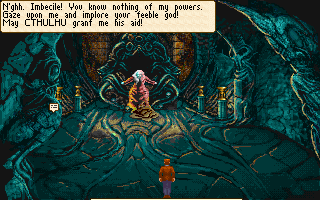
\includegraphics[scale=1]{shadow-comet.png}
  \end{center}
  \caption{Shadow of the Comet (DOS, 1993), realizado por la compañia francesa Infogrames}
    \label{fig:shadow-comet}
\end{figure}

Sin embargo, no sería hasta 1989, con el lanzamiento de Indiana Jones and the Last Crusade: The Graphic Adventure \cita{indiana-jones} de LucasArts, cuando se pondría este género de moda. Llegó la \cursiva{Edad de Oro} de las aventuras gráficas. Con la aparición de los CD-ROM se podían crear aventuras cada vez más largas y con mejores gráficos, incluso algunos incorporaban elementos 3D pre-renderizados y vídeos de imagen real.Grandes aventuras, en su gran mayoría de LucasArts, marcaron este inicio de la década de los 90, tanto que algunas acabaron como iconografía de la cultura popular y en los anales de la historia de los videojuegos. Una de las más destacadas fue The Secret of Monkey Island \cita{monkey-island} (1990) al centrarse más en la exploración y que el protagonista no pueda morir. Otra fue Day of the Tentacle \cita{day-tentacle} (1993), secuela de Maniac Mansion, que logró tal éxito que con las ganancias le permitió al director del apartado de diseño, Tim Schafer \cita{tim-schafer}, producir el videojuego exitoso Full Throttle \cita{full-throttle} incorporando las voces de Roy Conrad y Mark Hamill.

Sierra Online, por su lado, seguía con sus sagas populares Space Quest y King's Quest. Les mejoró su interfaz \cursiva{point-and-click} por una más amigable para el jugador, sin necesidad de introducir texto. No obstante, algunas de sus aventuras más reconocidas no llegaron a ser las de estas sagas, tal como pasó con Leisure Suit Larry in the Land of the Lounge Lizards \cita{larry-lizards} (1987, remake: 1991) que ganó en 1987 el premio al ``Mejor Juego de Aventura'' de la \cursiva{Software Publishers Association}.

%\begin{figure}[H]
%  \begin{center}
%    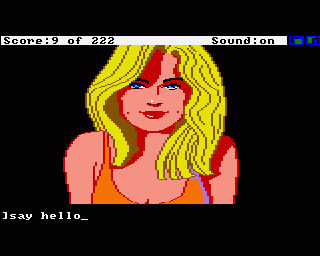
\includegraphics[scale=1]{larry-lizards.png}
%  \end{center}
%  \caption{Leisure Suit Larry in the Land of the Lounge Lizards (1987, remake: 1991)}
%    \label{fig:larry-lizards}
%\end{figure}

Lamentablemente, esta \cursiva{Edad de Oro} duró pocos años. A finales de los años 90, el público empezó a desviar sus miradas con las mejoras gráficas y de jugabilidad en los ordenadores. Aparecieron juegos dedicados más a la acción como los shooters en primera persona, y con el asentamiento de internet en los primeros hogares, los juegos online. Las aventuras gráficas poco podían hacer con estos avances, pues su mecánica hace que sean irrelevantes, y su popularidad y ventas cayeron. Así que los editores fueron cada vez más reacios a financiar aventuras gráficas por miedo a malas ventas.

Tal fue la crisís, que Sierra Online casi cerró completamente y LucasArts dejó de publicar después del año 2000. Hubo unas cuantas perlas antes del declive, Broken Sword: The Shadow of the Templars \cita{broken-sword} (1996) o Grim Fandango \cita{grim-fandango} (véase la figura ~\ref{fig:grim-fandango}), siendo este último un fracaso en ventas a pesar de ser aclamado por la crítica y algunos videojuegos más que no mencionaremos.

%\begin{figure}[H] 
%  \begin{center}
%    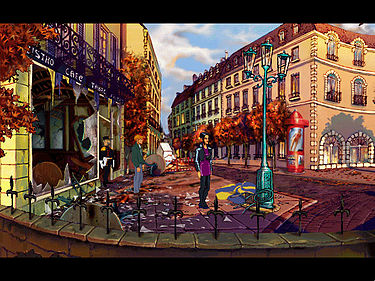
\includegraphics[scale=1.1]{broken-sword.jpg}
%  \end{center}
%  \caption{Broken Sword: The Shadow of the Templars (1996), una gran aventura gráfica en las que sus secuelas no estuvieron a su altura}
%    \label{fig:broken-sword}
%\end{figure}

\begin{figure}[H] 
  \begin{center}
    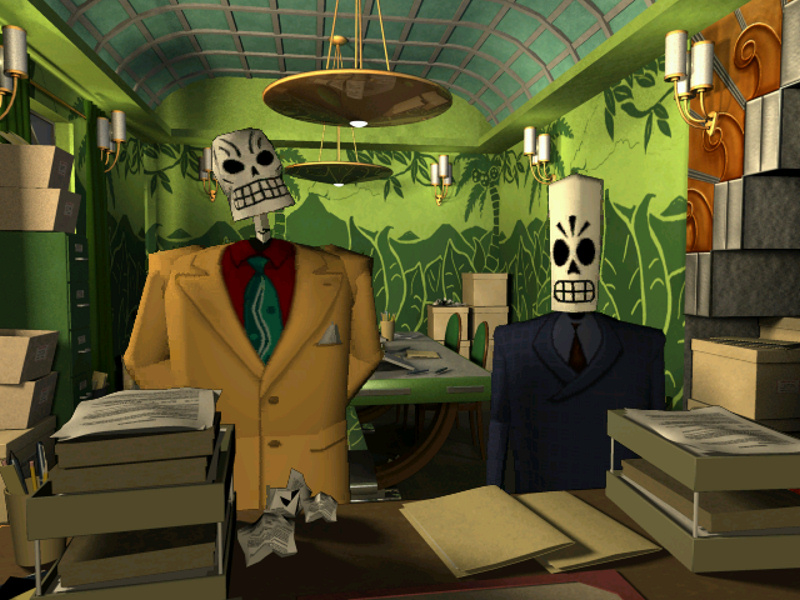
\includegraphics[scale=1]{grim-fandango.jpg}
  \end{center}
  \caption{Grim Fandango (1998), hecha íntegramente en 3D sin la clásica interfaz \cursiva{point-and-click}}
    \label{fig:grim-fandango}
\end{figure}

Después, si bien de manera independiente o amateur se fueron haciendo pequeñas obras gracias al auge de Adobe Flash y su soporte en internet. El subgénero de "escapa de la habitación" fue el que más juegos en su haber tuvo en estos años. Sin embargo, eran muy cortas, rudimentarias y repetitivas, no llegando casi nunca al público. 

No fue hasta la llegada de otras nuevas tecnologías, el resurgimiento de este género. La Nintendo DS, y Wii, permitía interactuar con el juego de una manera similar a usar un ratón de ordenador. Como resultado, varios desarrolladores crearon nuevas aventuras gráficas para estas plataformas. Ejemplos de aventuras gráficas de estas plataformas incluyen Zack \& Wiki: Quest for Barbaro's Treasure \cita{zack-wiki} (2007) para Wii, Hotel Dusk: Room 215 \cita{hotel-dusk} (2006) para Nintendo DS, y un port de Broken Sword: The Shadow of the Templars (2009) también para Nintendo DS. 

\begin{figure}[H] 
  \begin{center}
    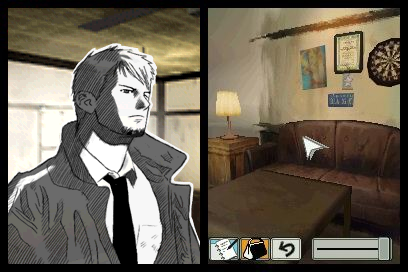
\includegraphics[scale=0.7]{hotel-dusk.png}
  \end{center}
  \caption{Hotel Dusk: Room 215 (2006), una aventura estilada como si fuera una novela negra}
    \label{fig:hotel-dusk}
\end{figure}

Pero sin duda, el verdadero renacer fue gracias a internet por asentarse totalmente en los hogares, y las mejoras de su velocidad a lo largo de estos años. Al fin era factible el poder promocionarte y distribuir tu juego sin costes intermedios, al menos dentro de un mercado de nicho. Una nueva compañía llamada Telltale Games \cita{telltale}, formada por antiguos miembros de LucasArts, empezó a producir nuevas aventuras gráficas para ordenador. Siguiendo una metodología de distribuir sus juegos de manera episódica, sus juegos incluyen Sam \& Max Save the World \cita{sam-max} (2006), Strong Bad's Cool Game for Attractive People \cita{strong-bad} (2008), el resurgir de Monkey Island con Tales of Monkey Island \cita{tales-monkey} (2009), Back to the Future: The Game \cita{back-future} (2010).

Su ópera prima llegó con el videojuego The Walking Dead \cita{walking-dead} (véase la figura ~\ref{fig:walking-dead}), aclamado tanto por la crítica como con el público. Su sistema de realizar decisiones difíciles en el momento y ver como influían en los personajes impactó enormemente, tanto que mucha gente hizo vídeos en Youtube de sus reacciones y elecciones, fomentando enormemente su difusión y su venta tanto en ordenador como en consolas.

\begin{figure}[H] 
  \begin{center}
    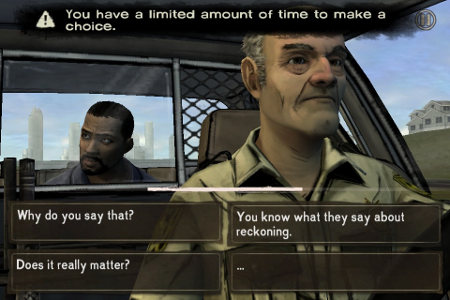
\includegraphics[scale=0.7]{walking-dead.jpg}
  \end{center}
  \caption{The Walking Dead (2012), su estética de cómic americano y su sistema de decisiones cautivó al público}
    \label{fig:walking-dead}
\end{figure}

No hay que olvidarse de otros muchos estudios independientes. Algunos optaron por seguir con las mecánicas clásicas, Machinarium \cita{machinarium} (2009) y Botanicula \cita{botanicula} (2012) de Amanita Designs son ejemplos de ello. Otras por mezclar mecánicas y nuevas tecnologías para reinventar las aventuras gráficas, como Dreamfall \cita{dreamfall} (2006), Portal \cita{portal} (2007) y muchos otros juegos, borrando las líneas del género. También podríamos incluir en este último, las películas interactivas por su semejanza con las aventuras gráficas, la más destacada Heavy Rain \cita{heavy-raiin} (2010) que fue un éxito de ventas.

Actualmente, sobre todo estos dos últimos años, el género está gozando una \cursiva{Edad de Plata}. Las redes nuevamente crearon un nuevo sistema de financiación, el crowdfunding (véase la siguiente sección), y se afianzaron las plataformas de distribución de videojuegos digitales, reforzando la presencia de estudios independientes y la creación de juegos que antes no se hubieran podido permitir. Una de las primeras en aprovecharse de este método, fue Double Fine Productions \cita{double-fine}. Junto con Tim Schafer, en febrero de 2012 lanzó una campaña en Kickstarter, la web de crowdfunding más famosa del mundo, para financiar Broken Age \cita{broken-age} (véase la figura ~\ref{fig:broken-age}). Causó un gran impacto, recaudando hasta la inmensa cantidad de 3,45 millones de dólares, confirmando el establecimiento del crowdfunding como una alternativa viable para financiar proyectos.

Una vez allanado el camino, otros estudios independientes siguieron la estela de Double Fine. AI Lowe, original creador de Leisure Suit Larry, lanzó una campaña para financiar un remake completo de su primera obra \cita{larry-reloaded}. 

\begin{figure}[H] 
  \begin{center}
    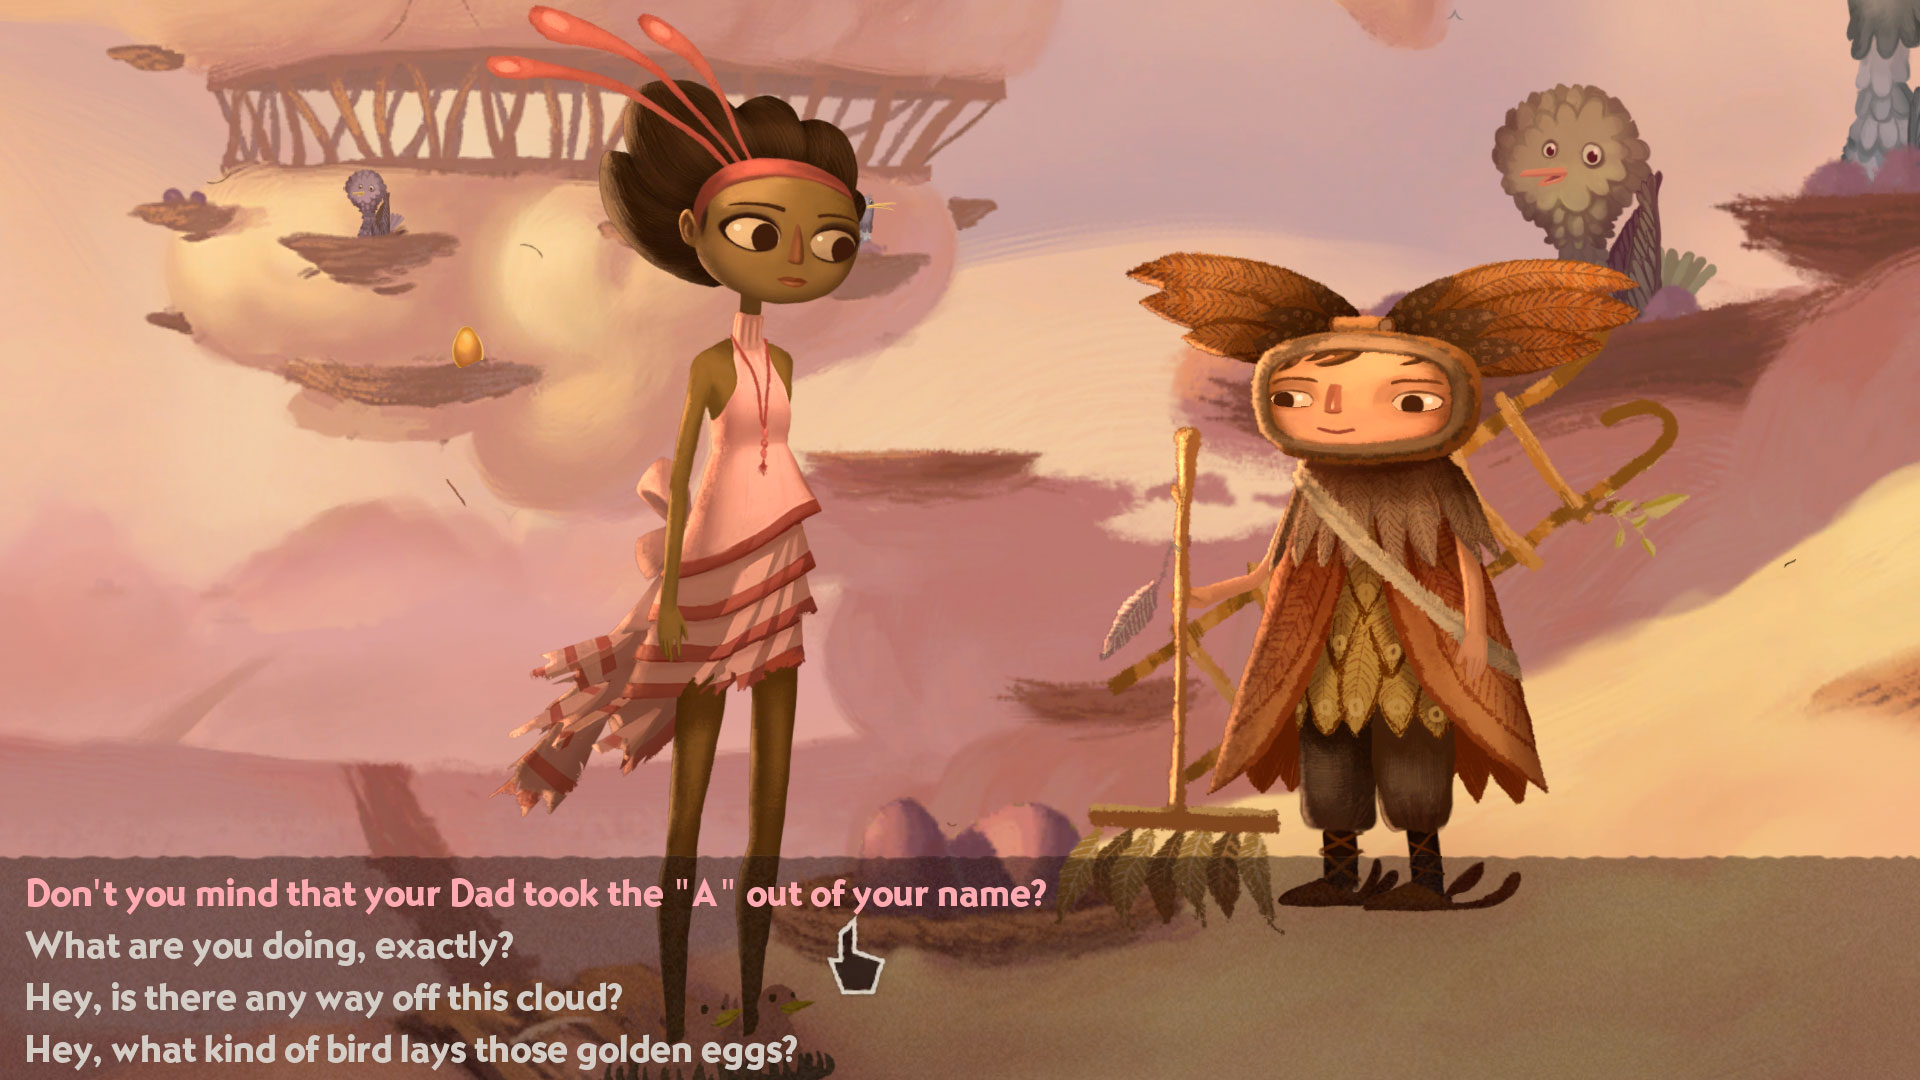
\includegraphics[scale=0.2]{broken-age.jpg}
  \end{center}
  \caption{Broken Age (2014), un cuento convertido en aventura gráfica financiada gracias al micromecenazgo}
    \label{fig:broken-age}
\end{figure}

Día a día, más estudios y empresas independientes se animan a lanzar sus aventuras gráficas. Y así gracias a las nuevas tecnologías y los estudios independientes, hemos recuperado este género olvidado.

¿Y qué pasó durante todos estos largos años en España? Pues en 1994 debutó Pendulo Studios \cita{pendulo} con la primera aventura gráfica española, Igor Objetivo Uikokahonia \cita{igor}. En 1997, lograría su mayor renombre con Hollywood Monsters \cita{hollywood-monsters}. Actualmente, son el mayor exponente del género en España con la saga Runaway \cita{runaway}. En 2011 ve la luz Hollywood Monsters 2 \cita{hollywood-monsters-2}, realizada enteramente en alta definición. Mientras que todos estos títulos siguen el más puro estilo clásico del género, el 29 de marzo de 2012, Péndulo lanzó New York Crimes \cita{new-york}, una aventura mucho más oscura y adulta de lo que sigue siendo el estilo clásico de las aventuras gráficas,  y la fusiona con la estética y composición propias del cómic.

\begin{figure}[H] 
  \begin{center}
    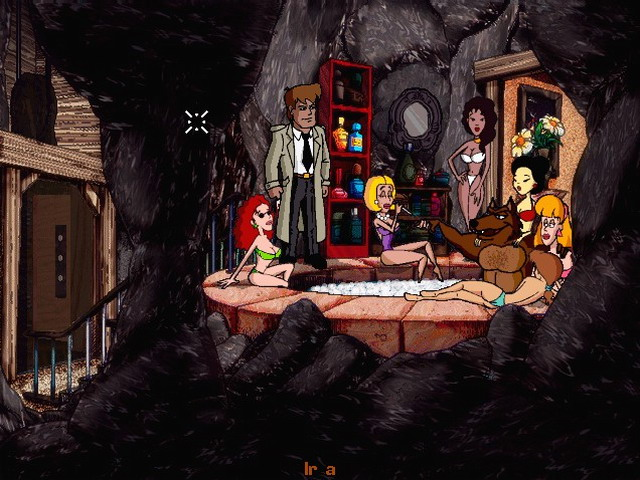
\includegraphics[scale=0.5]{hollywood-monsters.jpg}
  \end{center}
  \caption{Hollywood Monsters, la obra más remarcable de Pendulo Studios}
    \label{fig:hollywood-monsters}
\end{figure}

Aún así, pequeños estudios independientes españoles están empezando a hacer sus  pesquisas en este género. Dead Synchronicity \cita{dead-synchronicity} de Fictiorama Studios logró financiarse en abril del 2014, es un gran ejemplo de ello.

\subsection{Videojuegos en el ámbito educacional}
Un juego educativo (o ``juegos serios'' como se llaman actualmente), tal y como su nombre indica, es un juego diseñado con propósitos educacionales o que, de forma incidental o secundaria, tiene valor educativo. Cualquier juego ya sea en forma de juego de mesa, de cartas, o ser un videojuego puede ser usado, con el enfoque adecuado, en un ambiente educacional. Un juego educativo es un juego diseñado para enseñar a los humanos sobre una materia específica o habilidad. De hecho, cuando los educadores, gobiernos y padres se dieron cuenta de la necesidad psicológica y los beneficios de aprender jugando, esta herramienta educacional se extendió masivamente. Los juegos son una herramienta interactiva que, al utilizarlos, nos enseñan objetivos, reglas, resolución de problemas, interacción, todo representado como una historia.

El juego siempre ha sido una herramienta de aprendizaje para enseñar conceptos o habilidades nuevas. Antiguamente se usaban las parábolas y las fábulas para promover el cambio social, incluso en la Edad Media se enseñaba a jugar al ajedrez con el fin de enseñar a usar tácticas en las guerras. Pero lamentablemente, no existe mucha información concerniente a ello. No fue hasta el siglo XIX que el hombre empezó a tomarse en serio el uso de los juegos como una manera de enseñar con la creación de los jardines de infancia por Friedrich Fröbel, que basaba el aprendizaje mediante el juego. Los niños jugaban encantados con sus simples juegos educativos: bloques, kits de coser y materiales para tejer.

\begin{figure}[H] 
	\begin{center}
		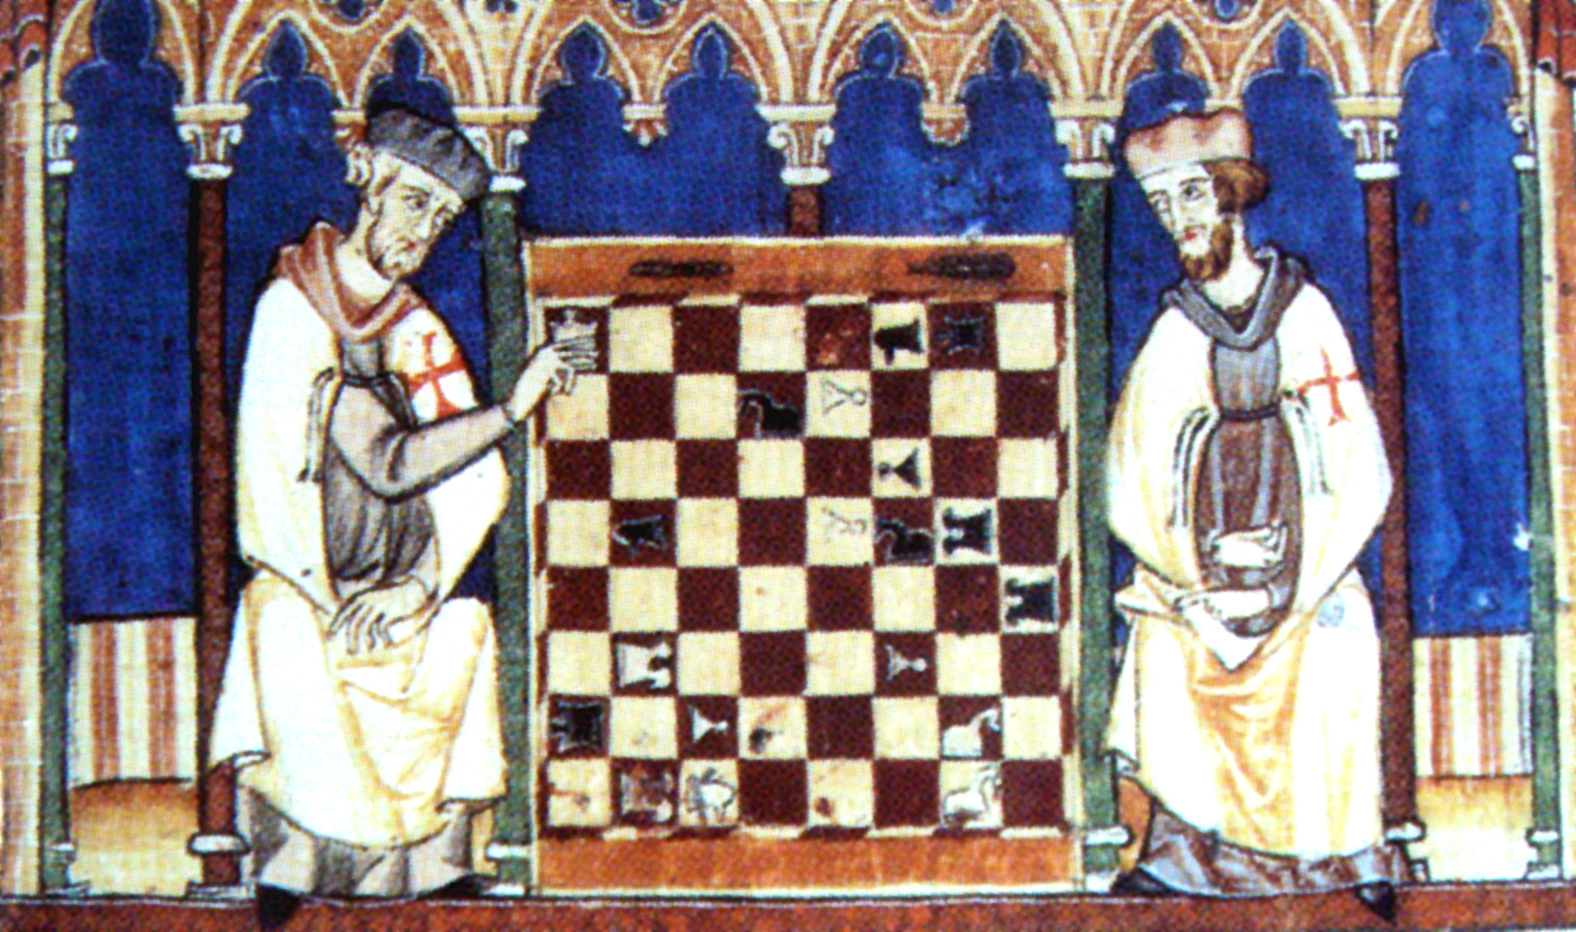
\includegraphics[scale=0.3]{ajedrez-edad-media.jpg}
	\end{center}
	\caption{Caballeros Templarios jugando al ajedrez, según el Libro de los Juegos (1283)}
	\label{fig:ajedrez-edad-media}
\end{figure}

Los juegos educativos fueron expandiéndose en diversas materias y creando juegos de mesas, cartas, etc. Pero no fue hasta la aparición de la tecnología en las casas, en la década de los 70, cuando Clark Abt propuso en su libro ``Serious Games''\cite{ccabt} una definición concreta de este tipo de juegos:

\emph{``Reducido a su esencia formal, un juego es una actividad entre dos o más personas con capacidad para tomar decisiones que buscan alcanzar unos objetivos dentro de un contexto limitado. Una definición más convencional es aquella en la que un juego es un contexto con reglas entre adversarios que intentan conseguir objetivos. Nos interesan los juegos serios porque tienen un propósito educativo explícito y cuidadosamente planeado, y porque no están pensados para ser jugados únicamente por diversión.''}

Aparte de esta definición, también se incluyó términos tales como ``juego educativo'', ``simuladores'', ``edutainment'' (entretenimiento educativo), etc. que años más tarde, se pondrían en práctica no solo en los juegos de mesa y cartas, sino también en la incipiente industria de los videojuegos. 

\begin{figure}[H] 
	\begin{center}
		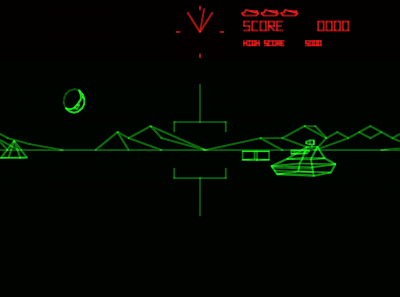
\includegraphics[scale=0.7]{army-battlezone-atari.png}
	\end{center}
	\caption{Army Battlezone tenía unos gráficos superiores a su época al ser en un principio de uso militar}
	\label{fig:army-battlezone-atari}
\end{figure}

Army Battlezone \cita{army-battlezone} se considera el primer videojuego dentro de la categoría de juegos serios, un proyecto fallido liderado por Atari en 1980, el cual fue diseñado para usar el videojuego arcade Battlezone como entretenimiento militar. Algunos juegos triunfaron también en el sector de los ``edutainment'' como fue el caso de ¿Dónde está Carmen Sandiego en el mundo? \cita{carmen-sandiego} (Apple II, 1985) que acabó convirtiéndose en los 90 en una franquicia de juegos, series de televisión y libros; o más tarde, la saga EcoQuest \cita{eco-quest} de Sierra Online o el de la aventura gráfica de La Pantera Rosa en Misión Peligrosa \cita{pink-panther} (PC, 1996). Pero a pesar de los esfuerzos de muchas compañías como Disney o Nintendo, la mayoría de ellos fueron un fracaso tras otro. Los juegos de entretenimiento educativo, no eran rentables. 

\begin{figure}[H] 
	\begin{center}
		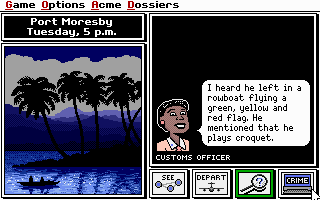
\includegraphics[scale=1]{carmen-sandiego-original.png}
	\end{center}
	\caption{¿Dónde está Carmen Sandiego en el mundo? fue uno de los pocos juegos educativos con éxito}
	\label{fig:carmen-sandiego}
\end{figure}

\begin{figure}[H] 
	\begin{center}
		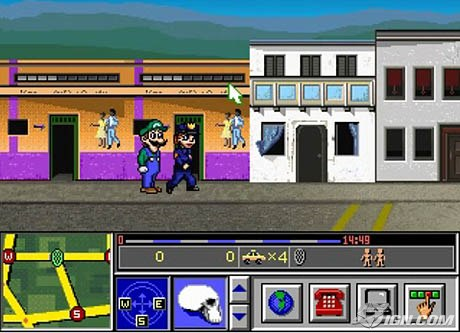
\includegraphics[scale=0.7]{mario-is-missing.jpg}
	\end{center}
	\caption{La saga Mario is Missing (MS-DOS, 1992) fue uno de los intentos fallidos por parte de Nintendo de realizar juegos educativos}
	\label{fig:mario-is-missing}
\end{figure}

Así que según fueron creciendo las capacidades técnicas de los juegos para proporcionar escenarios realistas, el concepto de juegos serios tuvo que ser reexaminado a finales de la década de los 90 con el fin de reorientar el camino de los juegos educativos. Durante este tiempo, algunos estudiosos comenzaron a examinar la utilidad de los juegos para otros propósitos, contribuyendo al creciente interés por emplearlos con nuevos fines. Además, la capacidad de los juegos para contribuir a la formación se vio ampliada con el desarrollo de los juegos multijugador. 

En 2002, el Centro Internacional para Académicos Woodrow Wilson creó la Serious Games Initiative \cita{serious-game-initiative} con el fin de fomentar el desarrollo de juegos sobre temas políticos y de gestión. Otros grupos más especializados aparecieron después en 2004, como por ejemplo Games for Change \cita{games-for-change}, centrado en temas sociales y en cambio social, y Games for Health, sobre aplicaciones relacionados con la asistencia sanitaria. Pero no se llegó a actualizar el término de juego serio.

Hasta 2005, no se abordó este término de una forma actualizada y lógica. Mike Zyda escribió artículo publicado en la revista ``Computer'' de la IEEE Computer Society que llevaba por título ``From Visual Simulation to Virtual Reality to Games''\cite{mzynda}. Zyda define primero el término de qué es un juego y luego continúa a partir de aquí:

\begin{itemize}
	\item \negrita{Juego}: una prueba física o mental, llevada a cabo de acuerdo con unas reglas específicas, cuyo objetivo es divertir o recompensar al participante.
	\item \negrita{Videojuego}: una prueba mental, llevada a cabo frente a una computadora de acuerdo con ciertas reglas, cuyo fin es la diversión o esparcimiento, o ganar una apuesta.
	\item \negrita{Juego serio}: una prueba mental, de acuerdo con unas reglas específicas, que usa la diversión como modo de formación gubernamental o corporativo, con objetivos en el ámbito de la educación, sanidad, política pública y comunicación estratégica.
\end{itemize}

Fue ampliamente aceptada por el público dicha definición, aunque no es la única para el término de "juego serio", pero se entiende que hace referencia a juegos usados en ámbitos como la formación, la publicidad, la simulación o la educación. Definiciones alternativas incluyen conceptos propios de los juegos y las tecnologías, así como nociones provenientes de aplicaciones no relacionadas con el entretenimiento. Los juegos serios empiezan a incluir también hardware específico para videojuegos, como por ejemplo de los videojuegos para mejorar la salud y la forma física (véase Wii Fit \cita{wii-fit}).

Los videojuegos son una herramienta a tener en cuenta en la estimulación cognitivo afectiva, que favorecen el aprendizaje, la autoestima, potencian la creatividad y las habilidades digitales, al mismo tiempo que generan motivación y entretenimiento. Los videojuegos suponen una modalidad de enseñanza que debe ser aprovecha por la comunidad educativa, por la cantidad de elementos emocionales que integran, su estimulación sensorial y la posibilidad de inmersión a través de los ambientes virtuales en los que se desenvuelven.

\begin{figure}[H] 
	\begin{center}
		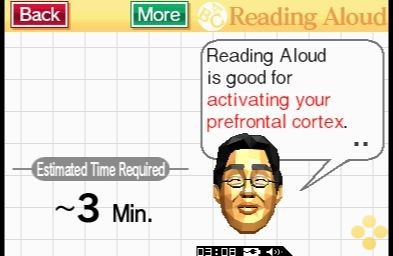
\includegraphics[scale=0.7]{brain-training.jpg}
	\end{center}
	\caption{Brain Training del Dr. Kawashima (Nintendo DS, 2005), un juego que estimulaba la mente para que pensáramos más rápido }
	\label{fig:brain-training}
\end{figure}

Los juegos serios están dirigidos a una gran variedad de público, desde estudiantes de educación primaria y secundaria a profesionales y consumidores. Los juegos serios pueden ser de cualquier género, usar cualquier tecnología de juegos y estar desarrollados para cualquier plataforma. Algunos lo consideran un tipo de entretenimiento educativo, aunque el grueso de la comunidad se resiste a este término.

Un juego serio puede ser una simulación con la apariencia de un juego, pero está relacionado con acontecimientos o procesos que nada tienen que ver con los juegos, como pueden ser las operaciones militares o empresariales. Los juegos están hechos para proporcionar un contexto de entretenimiento y autofortalecimiento con el que motivar, educar y entrenar a los jugadores. Otros objetivos de estos juegos son el marketing y la publicidad. Los grandes usuarios de los juegos serios parecen ser el gobierno de los Estados Unidos y los médicos. Otros sectores comerciales están también persiguiendo activamente el desarrollo de este tipo de herramientas.

\begin{figure}[H] 
	\begin{center}
		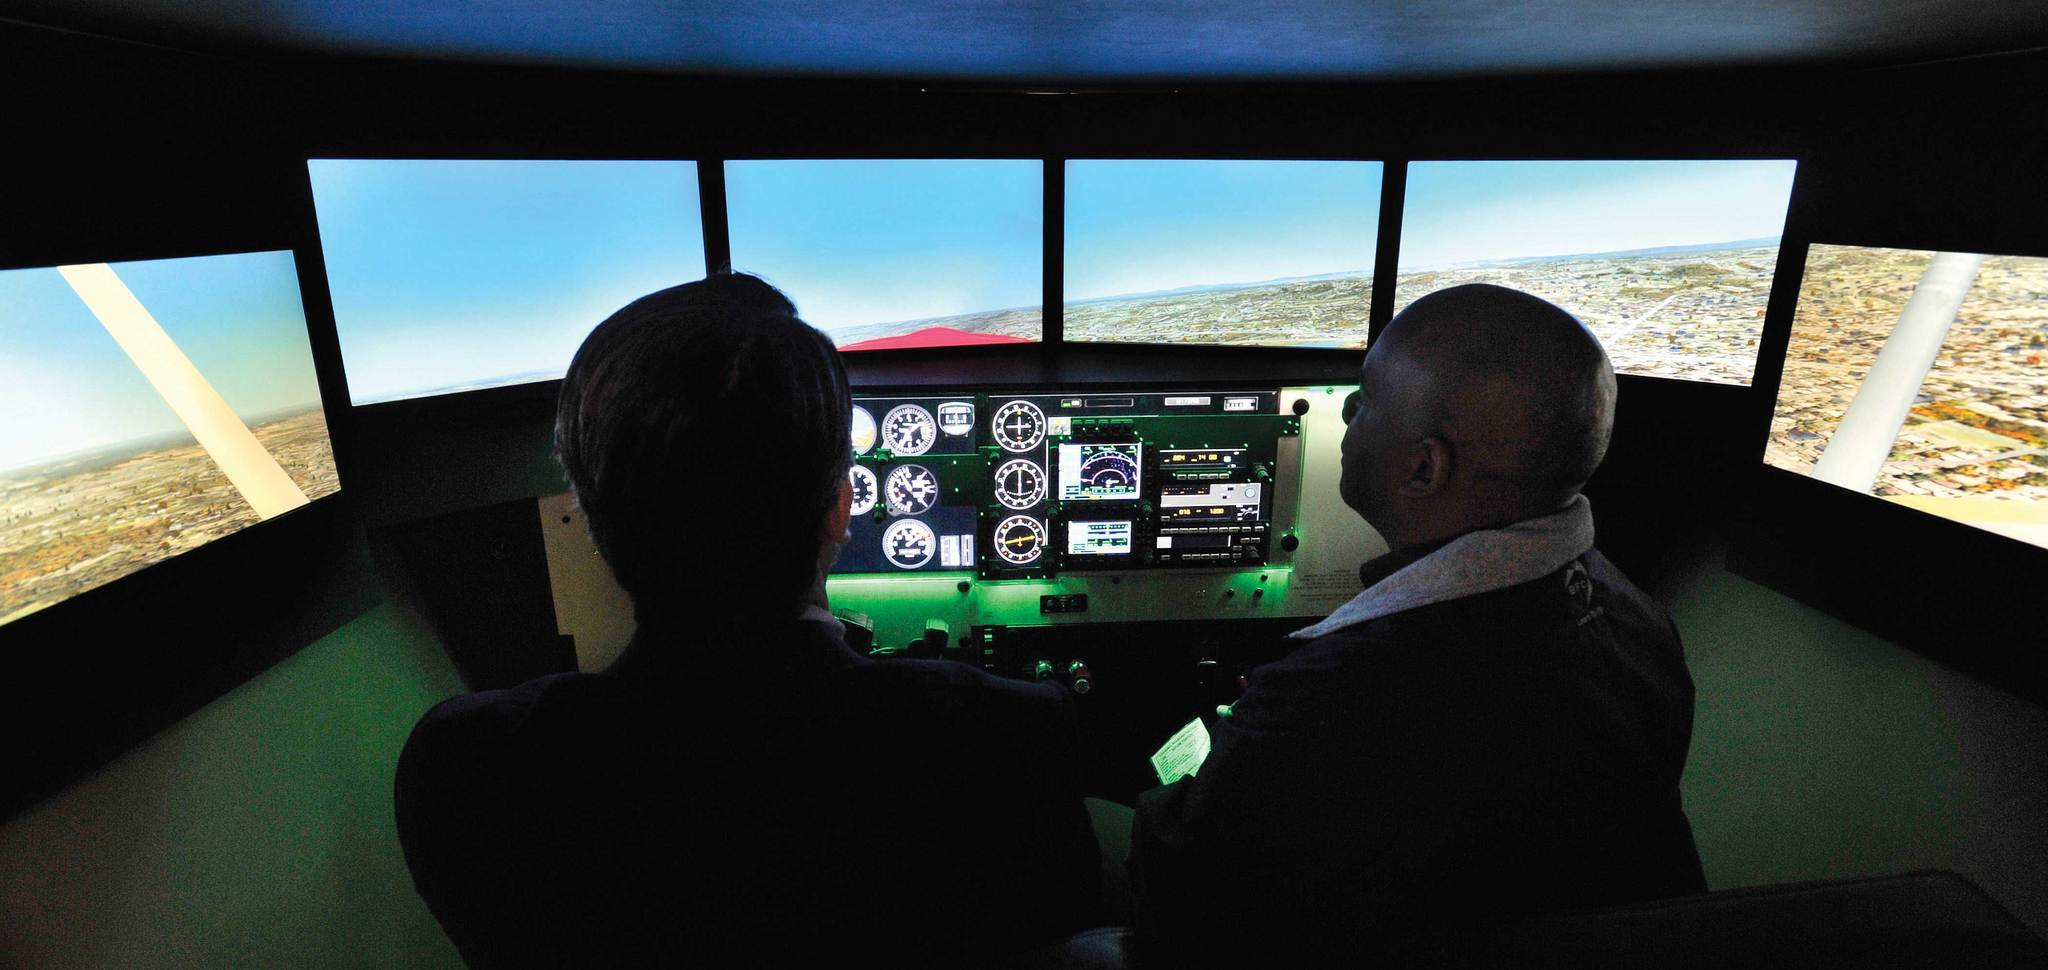
\includegraphics[scale=0.2]{simulador-vuelo-profesional.jpg}
	\end{center}
	\caption{Simulador de vuelo profesional para enseñar a los nuevos pilotos}
	\label{fig:simulador-vuelo}
\end{figure}

Actualmente existe una clasificación, más o menos aceptada pues no existe consenso oficial, de los juegos serios de acuerdo a su propósito:

\begin{itemize}
	\item \negrita{Advergames}: del inglés \emph{advertising} y \emph{game}, es decir, publicidad y juego, es la práctica de usar videojuegos para publicitar una marca, producto, organización o idea.
	
	\item \negrita{Edutainment}: este es un término que resulta de la unión de \emph{education} y \emph{entertainment}, es decir, educación y entretenimiento o diversión. Se aplica a los programas que enseñan mediante el uso de recursos lúdicos.
	
	\item \negrita{Aprendizaje basado en juegos}: del inglés \emph{educational game}, estos juegos tienen como objetivo mejorar el aprendizaje. Están diseñados en general manteniendo un equilibrio entre, por un lado, la materia y, por otro, la jugabilidad y la capacidad del jugador para retener y aplicar dicha materia en el mundo real. Este último tipo de juegos se utilizan en el mundo empresarial para mejorar las capacidades de los empleados en temas, atención al público y negociaciones.
	
	\item \negrita{Edumarket Games}: cuando un juego serio combina varios aspectos (por ejemplo, los propios del advergaming y del edutainment u otros relacionados con la prensa y la persuasión), se dice que la aplicación es un juego de tipo edumarket, término que resulta de la unión de \emph{education} y \emph{marketing}.
	
	\item \negrita{News Games}: son juegos periodísticos (del inglés \emph{news}, es decir, noticias) que informan sobre eventos recientes o expresan un comentario editorial.
	
	\item \negrita{Simuladores}: son juegos que se emplean para adquirir o ejercitar distintas habilidades o para enseñar comportamientos eficaces en el contexto de situaciones o condiciones simuladas. En la práctica, son muy usados los simuladores de conducción de vehículos (coches, trenes, aviones, etc.), los simuladores de gestión de compañías y los simuladores sobre negocios en general, que ayudan a desarrollar el pensamiento estratégico y enseñan a los usuarios los principios de la micro y macroeconomía y de la administración de empresas.
	\item \negrita{Juegos persuasivos}: del inglés \emph{persuasive games}, son juegos que se usan como tecnología de la persuasión para convencer a sus jugadores de que un concepto o idea está bien o mal.
	\item \negrita{Juegos organizativos dinámicos}: del inglés \emph{organizational-dynamic games}, son juegos que enseñan y reflejan la dinámica de las organizaciones a tres niveles: individual, de grupo y cultural.
	\item \negrita{Juegos para la salud}: del inglés \emph{games for health}, son juegos diseñados como terapia psicológica, o juegos para el entrenamiento cognitivo o la rehabilitación física.
	\item \negrita{Juegos artísticos}: del inglés \emph{art games}, son juegos usados para expresar ideas artísticas, o arte creado, utilizando como medio los videojuegos.
	\item \negrita{Militainment}: es un término de la unión de \emph{military} y \emph{entertainment}, es decir, militar y entretenimiento o diversión. Son juegos financiados por el ejército o que, de lo contrario, reproducen operaciones militares con un alto grado de exactitud. Lamentablemente, en su mayoría son privados para el público general dado el secretismo militar sobre para qué lo usan y cómo lo usan.
\end{itemize}

Cómo conclusión, podemos decir que si actualmente los juegos serios se han separado bastante de los videojuegos como medio de entretenimiento, aún siguen perdurando juegos de la gama de edutainment que intentan aunar estos dos campos. Pero lo que si podemos decir con certeza es que los primeros videojuegos educativos eran en su mayoría aventuras gráficas tal y como se ha visto en los ejemplos dados. No es difícil de saber el por qué, las aventuras gráficas, tal y cómo se describen en la sección anterior, son juegos dedicados a resolver problemas de lógica. Al recurrir más al esfuerzo mental que otros juegos que buscan los reflejos motores en los jugadores, es fácil realizar conexiones lógicas con las que enseñar datos concretos de forma que acabemos asociándolos a la realidad y aprendamos.

%\newpage
\section{Motivaciones}
\label{sec:motivaciones}
Comenzar a usar una tecnología desconocida como \programa{Unity3D}, aprender un nuevo lenguaje como C\# junto con la API de \programa{Unity3D} para este lenguaje, o cualquier otra, siempre entraña dificultad y, si le añadimos la documentación histórica para contrastar que toda la información que se presente tanto en esta memoria como en el videojuego final será verídica, aún más. La principal motivación para embarcarse en la confección de este proyecto, es la de la capacidad que existe en un videojuego tanto para entretener, transmitir sentimientos, ideas y emociones, como para ser una herramienta de apoyo a la enseñanza en prácticamente cualquier ámbito que se proponga la industria.

Diseño de Videojuegos era una asignatura optativa de tercer curso de la extinta titulación Ingeniería Técnica de Informática de Sistemas dentro de la Universidad de Cádiz. En dicha asignatura los alumnos se organizaban en grupos de tres alumnos con el objetivo de desarrollar un juego sencillo durante el cuatrimestre. Las únicas restricciones eran que el videojuego resultante debe ser completamente libre y que se había de utilizar la forja de código de RedIRIS \cita{rediris} junto a Subversion \cita{subversion} como sistema de control de versiones. Los alumnos escogían bibliotecas, usualmente libres, para el desarrollo de aplicaciones multimedia en dos dimensiones como libSDL \cita{sdl} o Gosu \cita{gosu}. Toda la documentación estaba en inglés, pero por suerte ya se publicó una excelente documentación en castellano en formato wiki llamada Wikijuegos \cita{wikijuegos} para libSDL.

Dicha asignatura era casi totalmente enfocada a aprender a programar y el diseño era algo más secundario, limitándose a unas pocas páginas que definieron a grandes rasgos los elementos que iban a desarrollarse en el juego.

Lamentablemente mucha, prácticamente toda la documentación sobre el diseño de juegos con una complejidad alta o mediana está en inglés. Poniendo por ejemplo el caso de documentos de diseño de aventuras gráficas, las cuales son orientadas más al contenido narrativo y varían el diseño general por uno más específico para puzzles, solo se pueden encontrar liberados documentos de puzzles y/o diseño en este idioma, siendo las más destacadas la de Grim Fandango \cita{grimfandango_doc}, las aventuras clásicas de AI Lowe \cita{ailowe_doc} y alguna que otra reciente como la de Resonance en foros de AdventureGameStudio \cita{resonance_doc}. Con todo esto, una de mis principales motivaciones es la de crear un documento de diseño extrapolable a todos los géneros, y aparte un documento de diseño de puzzles, todo esto en español y lo más completa posible, para que sirva de ejemplo para desarrolladores de videojuegos de habla hispana.

Por otra parte, dejando de lado el diseño, lo mismo se puede decir de ejemplos de código en español de aventuras gráficas. \programa{Unity3D} es una herramienta ideal para ello, pues es la más usada actualmente para iniciarse en el mundo del desarrollo de videojuegos, además de ser ampliamente usada por estudios por su versión gratuita y la variedad de plataformas en las que se puede compilar con un único código. Así pues, una motivación es la de generar un juego completo con el código documentado dividido en bloques reutilizables.

La ubicación de la Universidad de Cádiz y el pasado histórico su ciudad fue otra motivación, pues cuando empezaba con las dudas de sobre qué proyecto iba a realizar, se celebró el Bicentenario de la Constitución de 1812. Proporcionándome la idea de dar a conocer cómo es Cádiz y su historia del 1812, tanto para residentes de Cádiz, como españoles y extranjeros que nunca hayan visitado Cádiz.

Es posible resumir las motivaciones que me han llevado a desarrollar este proyecto en cubrir el vacío de documentación y la falta de proyectos completos en castellano, y el deseo personal de aprender a diseñar videojuegos.

%\newpage
\section{Objetivos}
\label{sec:objetivos}
El objetivo del proyecto viene extraído de forma lógica de las motivaciones (sección~\ref{sec:motivaciones}). Con \nombrejuego se pretende crear un juego ampliamente documentado y accesible que sirva de referencia para futuros desarrolladores de videojuegos españoles. Deberá debe cumplir con los siguientes requisitos:

\begin{itemize}
\item Servir de ejemplo lo más cercano a la realidad posible de lo que es un diseño medianamente complejo de un videojuego. Es muy habitual terminar de leer documentación, realizar diseños sencillos para pequeños juegos pero que a la hora de embarcarse a un proyecto con más complejidad es necesario organizarlo y esquematizarlo bien o acabaremos con un videojuego que no tiene ni pies ni cabeza. Para eso es imprescindible que se documente cada fase del desarrollo.
\item Crear un sistema intermediario entre el videojuego y el texto de los diálogos, de forma que, al ser independiente el texto, se pueda modificar sin interferir con el código, e incluso poder crear traducciones sin afectar en nada al mismo. Este sistema debe ser reutilizable y estar bien documentado.
\item Crear una Base de Datos con información histórica y un buscador dentro del juego para acceder a ella. El motivo de esto es el poder acceder a los datos de manera rápida y sencilla para poder seguir avanzando en el juego sin problemas.
\item Convertirse en un ejemplo de trabajo con un equipo multidisciplinar. En un videojuego profesional deben trabajar juntos desde unas pocas personas hasta varios centenares por lo que la coordinación entre profesionales de distintas áreas es muy importante. Será necesario encontrar artistas relacionados con la animación e ilustración, música y efectos de sonido.
\item No sólo debe ser útil a los interesados en el desarrollo sino también de cara al usuario final. \nombrejuego debe de ser intuitivo, divertido y útil para ayudar a asimilar datos, en este caso históricos.
\item Crear subsistemas independientes del videojuego reutilizables. Por supuesto, deben venir acompañados de la documentación pertinente: dependencias, instalación, uso y licencia.
\end{itemize}

\subsection{Sobre este documento}
La presente memoria de \negrita{Proyecto fin de Carrera} posee la siguiente estructura en capítulos y apéndices:

\begin{itemize}

\item En el capítulo~\ref{chap:introduccion} que actualmente nos ocupa, se hace una breve introducción sobre el contexto en el que nos situamos. Se ofrece una visión del mundo de la industria de videojuegos, principalmente independiente, se habla sobre las aventuras gráficas, que es el género en el que se va a basar \nombrejuego y la importancia de dicho género en el ámbito educativo. Finalmente se evidencia la necesidad de documentación en cuanto a diseño de videojuegos medianamente complejos en castellano y se adjuntan el resto de motivaciones y objetivos relacionados con el proyecto.

\item En el capítulo~\ref{chap:planificacion} se expone la organización temporal de todo el desarrollo a través de un diagrama de Gantt. Más adelante se comenta brevemente cada una de las tareas que conforman la planificación.

\item En el capítulo 3 se refleja el proceso de desarrollo para el videojuego \nombrejuego. Comenzando con el documento de diseño, el documento de puzzles, se sigue con la fase de análisis, diseño e implementación. Se hace especial hincapié en el sistema intermediario del texto con el juego, y la base de datos e introducción en el juego. Se finaliza con las pruebas realizadas.

\item En el capítulo 4 se hace una breve reflexión personal seguida de otra técnica tratando de aglutinar los conceptos aprendidos, la riqueza que ha proporcionado la experiencia y lo que podrá aportar tanto a usuarios como desarrolladores. Finalmente termina con un pequeño listado sobre las posibilidades de ampliación del proyecto.

\item En el apéndice Software utilizado se hace un repaso por todas las herramientas empleadas a lo largo del desarrollo del proyecto. Asimismo, se adjuntan comentarios y razones de uso.

\item En el apéndice Manual de usuario se incluye un completo manual de usuario para \nombrejuego. El documento contiene la introducción a la historia, personajes y lugares así como una completa guía de instalación en sistemas GNU/Linux y Windows. Posteriormente se detallan las mecánicas de juego y los controles en detalle. Finalmente se añade una completa guía para añadir traducciones adicionales a \nombrejuego usando el lenguaje XML.

\end{itemize}
